%----------------------------------------------------------------------------
\chapter{\AudioOverIp}
%----------------------------------------------------------------------------
\section{Bevezetés az Audio over IP világába}
%----------------------------------------------------------------------------
A 1990-es évek végén a szakmai hangipar jelentős elmozduláson ment keresztül, amikor a pont-pont digitális 
átvitel formátumokról, mint az AES/EBU és a MADI, áttért az IP-alapú szabványokra, például az AES67-re. 
Ez a csomag alapú hálózati megoldás jelentős rugalmasságot és kibővített vezérlési valamint monitorozási 
képességeket biztosít a hangrendszerek számára. Lehetővé teszi, hogy egy már meglévő telepítés későbbi 
szoftverkonfigurációkkal és frissítésekkel alkalmazkodóvá és bővíthetővé váljon. 
A gyártók ezen felül új funkciókkal is kiegészíthetik a meglévő eszközöket különböző esetekben.

Az IP-alapú megközelítésnek köszönhetően a jelutak már nem kötődnek szoros 
kapcsolatban a fizikai kábelekhez; a jelátviteli utak bármikor egyszerű egérkattintásokkal módosíthatók, 
elkerülve a fizikai átrendezést vagy dedikált audio útválasztó hardverek szükségességét. 
A csomagorientált átvitel természeténél fogva az audiojelek automatikusan eljutnak a kívánt helyre az IT hálózaton keresztül.

Az első sikeres audio-over-Ethernet hálózatmegoldásként általában a Cirrus Logic által 1996-ban bevezetett 
CobraNetet tartják számon. Számos audio telepítés alapját képezi, beleértve kongresszusi központokat, színházakat, koncerttermeket, repülőtereket és vidámparkokat. Bár a CobraNet még ma is széles körben alkalmazott, magas késleltetési problémái és korlátozott mérethatékonysága miatt nem ideális választás élő hangrendszerek, stúdiófelvételek és rádió létesítmények számára.

Körülbelül tíz évvel később az ausztrál Audinate cég által kifejlesztett Dante, 
amely a „Digital Audio Network Through Ethernet” rövidítése, új szintre emelte az audio-over-IP technológiákat. A Dante számos jelentős előnnyel rendelkezik az első generációs technológiákhoz képest, beleértve a jobb használhatóságot és a magasabb kompatibilitást a szabványos hálózati infrastruktúrákkal. A Dante hatalmas hardveres ökoszisztémára épít, amely több ezer eszközt tartalmaz, különböző gyártóktól.

A Dante domináns pozícióját megelőzően az AVB (Audio Video Bridging) nevű technológia 
körüli várakozások is jelentősek voltak. 
Az AVB technológiát más iparágak, mint például az autóipar és az ipari automatizálás is átvették, 
és általánosabb néven ismerték el, mivel nem csupán hang- és videóalkalmazásokhoz kapcsolódik. 
Az AVB-t a gyártók fejlesztőcsoportja, az AVnu Alliance, időérzékeny hálózat (TSN - Time Sensitive Network) néven ismerte el.

Ezt követően a Milan munkacsoport, amely audio/video gyártókból álló konzorcium, kidolgozott egy 
finomhangolt specifikációt a professzionális audio/video rendszerek számára, amely Milan néven ismert. 
Ez a specifikus TSN verzió az audio/video szolgáltatók közötti interoperabilitásra összpontosít.

%----------------------------------------------------------------------------

Az IP-alapú hálózatokra való átállás az analóg hangról digitális hangra való áttéréssel vonható párhuzamba. 
Az átmeneti időszakban kezdetben csupán néhány telepítés használta az új technológiát, ami kezdetben problémákat okozhatott a kezelés vagy a megbízhatóság terén, összehasonlítva a hagyományos, régebbi megoldásokkal. 
Ezek a problémák azonban a technológia fejlődésével fokozatosan megszűnnek.

Az IT hálózatok működése több szempontból eltér a hagyományos audio útválasztási módszerektől. 
Először is, a standard IT hálózatok nem úgy vannak kialakítva, hogy szigorú időzítési 
követelményeket teljesítsenek, amelyek az audio alkalmazások esetében jellemzőek. 
Egy hálózati környezetben az adatcsomagok útját más csomagok is akadályozhatják, ami 
jelentős időbeli eltéréseket okozhat az érkezési időben. Ezzel szemben a hagyományos 
audio kábelek esetében az adatok továbbításának időzítése nem változik meg a kábel mentén.

Másodszor, az IT alkalmazásoknál egy csomag elvesztése általában elfogadható, mivel az 
elveszett adatcsomagokat automatikusan újraküldik. Az audio alkalmazásokban azonban a 
késleltetés minimalizálása érdekében elengedhetetlen, hogy a csomagok első alkalommal a 
megfelelő helyre érkezzenek, mivel nincs elegendő idő az újraküldéshez. Ha néhány csomag 
elveszik, az azonnali megszakításokat és kimaradásokat okozhat, amelyek hallhatóak.

A csomagvesztés egyik gyakori oka a hálózati linkek túlterheltsége, illetve a túl alacsony pufferméret. 
Az audiohálózatokat úgy kell tervezni, hogy elegendő sávszélesség álljon rendelkezésre minden felhasználó 
számára egyidejű használat esetén is. Amennyiben ez a feltétel teljesül, és a csomagkiszállítás időben történik, ahogy az audio alkalmazások megkívánják, a hálózat elméletileg hosszú távon stabilan működhet.

Mindezek ellenére célszerű a hálózatot túlbiztosítani úgy, hogy minden csomag időben 
megérkezzen, elkerülve a további finomítások szükségességét a kapcsolók konfigurációjában. 
Ez konkrétan azt jelenti, hogy olyan IT hálózatokat kell kialakítani, amelyek elegendő 
sávszélességgel rendelkeznek és kizárólag audio alkalmazások számára vannak fenntartva, 
elkerülve, hogy azok általános mindennapi alkalmazásokkal keveredjenek.

%----------------------------------------------------------------------------

Az audio-over-IP technológiák többsége azon alapfeltevésre épít, hogy a háttérben működő hálózat megbízhatóan teljesít. 
Ez magában foglalja a csomagvesztés teljes hiányát és a súlyos csomagütközések elkerülését a kapcsoló hardveren. 
Bizonyos hálózatokban, különösen olyan esetekben, amikor az audio forgalmat más típusú forgalommal, például 
internetes böngészéssel kombinálják, kiemelt jelentőséggel bírhat az audio és szinkronizációs csomagok elsőbbségi kezelése. 
Ennek célja, hogy az audio adatok zavartalanul érkezzenek meg, minimalizálva a késleltetést és biztosítva a megfelelő szinkronizációt. 
Ezt a funkciót a legtöbb modern kereskedelmi forgalomban elérhető kapcsoló támogatja. \newline

Példa audio over IP hálózatokra:
%----------------------------------------------------------------------------
\begin{itemize}
	\item Audinate által kifejlesztett - Dante
\end{itemize}
\begin{itemize}
	\item QSC által kifejlesztett - Q-LAN
\end{itemize}
\begin{itemize}
	\item Lawo és Partnerei által kifejlesztett - RAVENNA
\end{itemize}
%----------------------------------------------------------------------------
\begin{figure}[H]
	\centering
	
\includegraphics[width=50mm, keepaspectratio]{figures/dante_logo.jpg}
	\caption{Audinate Dante logó}
	\label {fig:dante_logo}
\end{figure}
%----------------------------------------------------------------------------
\subsection{Előnyök és hátrányok}
%----------------------------------------------------------------------------
Az IT hálózatok alkalmazása hangkapcsolatokra nézve számos előnyt kínál:
\begin{itemize}
	\item Rugalmasság hangkapcsolatok hozzáadásához vagy módosításához anélkül,
	      hogy kábeleket cserélnénk.
\end{itemize}
\begin{itemize}
	\item Viszonylag alacsony áron széles skálájú funkciókat kínál.
\end{itemize}
\begin{itemize}
	\item Alkalmazkodás és integráció az IT hálózati infrastruktúrákba
	      specifikus audio vagy videokábelek alkalmazása nélkül.
\end{itemize}
\begin{itemize}
	\item Videójel és vezérlési adatok továbbíthatók ugyanazon infrastruktúrán
	      keresztül.
\end{itemize}
%----------------------------------------------------------------------------
Ugyanakkor az audio-over-IP hálózatok felhasználóit számos kihívás elé is állíthatják:
%----------------------------------------------------------------------------
\begin{itemize}
	\item Azért mert általában több hangmintát egy csatornából egy csomagba helyeznek
	      el a hatékonyság érdekében, adott minimális késleltetés adódik, mivel az
	      küldőnek meg kell várnia, hogy a hangminták rendelkezésre álljanak, mielőtt
	      azokat átküldené a hálózaton. Ez a késleltetés általában magasabb, mint a
	      pont-pont digitális hangszabványok esetében, de optimalizált csomagformátumok és
	      hálózati beállítások segítségével minimalizálható és nagyon jól közelíthető.
\end{itemize}
\begin{itemize}
	\item Mivel az IT hálózatok nem meghatározottak a csomagok út idejét tekintve,
	      egy biztonsági tartományt, azaz egy audio buffer-t kell beszúrni a fogadó végén.
	      Ez a buffer további késleltetést eredményez. Minél kevesebb csomagütközés van
	      jelen a hálózatban, annál inkább csökkenthető ez a biztonsági tartomány és
	      ezzel a késleltetés.
\end{itemize}
\begin{itemize}
	\item Az audio csomagformátumok változatossága miatt növekszik a komplexitás,
	      ami azt jelenti, hogy a fogadóknak és küldőknek azonos beállításokkal kell
	      rendelkezniük. Az audio-over-IP technológia komplexitása jelentősen magasabb,
	      mint az előző technológiáké. Az iparág még mindig jelentős munkát végez annak
	      érdekében, hogy csökkentse ezt a komplexitást a felhasználók számára, bevezetve
	      intelligens és felhasználóbarát szoftvermegoldásokat az audiohálózatok
	      kezelésére.
\end{itemize}
%----------------------------------------------------------------------------
\subsection{Fázishelyesség}
%----------------------------------------------------------------------------
Az audio alkalmazások esetében kritikus jelentőségű a több eszköz szinkronizált működése, különösen a mikrofonok és hangszórók közötti fázispontosság biztosítása. Amennyiben egy erősítőhöz több hangszóró csatlakozik, és az összes csatorna egyetlen hangcsomagban érkezik, nincs veszélye annak, hogy a csatornák egymással ellentétes fázisban működjenek, mivel a hangminták az átvitel során nem változnak el egymáshoz képest.

Azonban a modern alkalmazásokban, ahol több erősítő és processzor függetlenül kap hangcsomagokat, 
továbbra is szükség van arra, hogy az audiojeleket pontos fázispontossággal reprodukálják. 
Ennek érdekében az audio csomagokat több hálózati eszköz is fogadhatja, pufferelheti és azonos időben kell lejátszania őket.

Mivel az IT hálózatok nem rendelkeznek szigorú időzítési előírásokkal a csomagok továbbításának és 
megérkezésének időpontjára vonatkozóan, az audiohálózatoknak szinkronizációs megoldásokat kell alkalmazniuk. 
Ez új kihívást jelent az audio-over-IP technológiák számára, amelyet minden ilyen rendszernek kezelnie kell.

Az audiohálózaton belül minden eszköznek pontosan szinkronizált állapotban kell lennie a Precision Time Protocol (PTP) szabvány szerint. 
Ez azt jelenti, hogy az eszközök belső órái (PTP követők) egy referenciaórából (PTP vezető) származnak. 
A referenciaóra lehet bármelyik audioeszköz, amely támogatja ezt a funkciót, vagy egy kifejezetten erre 
a célra tervezett készülék, amely pontos PTP órát biztosít. A vezető eszközt felhasználói beállítások 
vagy automatizmus választja ki. Minden eszköz, legyen az audio adó vagy vevő, végső soron az adott 
időhöz való pontos szinkronizációt követeli meg.

A hangcsomag küldési időpontját időbélyegzővel látják el. A felhasználó egy állandó 
időeltolást, úgynevezett linkeltolást, állít be az összes vevőnél. Amikor egy csomag 
megérkezik egy vevőhöz, a pufferben tárolódik, amíg le nem játszák. 
Így az audio lejátszási időpontja a küldési idő és a linkeltolás összegeként határozható meg. \newline

Minden vevő két feltétel mellett érheti el egymás között a fázispontosságot:
%----------------------------------------------------------------------------
\begin{itemize}
	\item Pontos időszinkronizálás a PTP óra vezetőjéhez (azonos időbázis).
	\item Azonos linkeltolási érték beállítása a felhasználó által az összes vevőeszközön.
\end{itemize}
%----------------------------------------------------------------------------

A linkeltolást az érintett összes kapcsolat legrosszabb esetű késleltetése alapján kell meghatározni. 
Javasolt, hogy a váratlan csomagkiszállítási idők eltérései miatt egy kis engedményt is 
beiktassunk, ami azt jelenti, hogy valamivel hosszabb időt kell biztosítani az átlagos csomagfeldolgozási időnél. 
Ez a megközelítés széles körben elterjedt, és jelenleg minden audiohálózati szabványban alkalmazásra kerül.

%----------------------------------------------------------------------------
\begin{figure}[H]
	\centering
	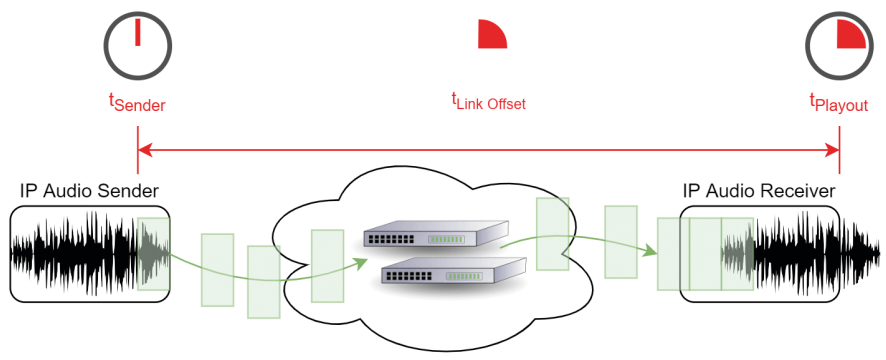
\includegraphics[width=\linewidth, keepaspectratio]{figures/link_offset_latency.png}
	\caption{A kapcsolati eltolás meghatározza a késleltetést \cite{AHNERT2023}}
	\label {fig:link_offset_latency}
\end{figure}
%----------------------------------------------------------------------------
\begin{figure}[H]
	\centering
	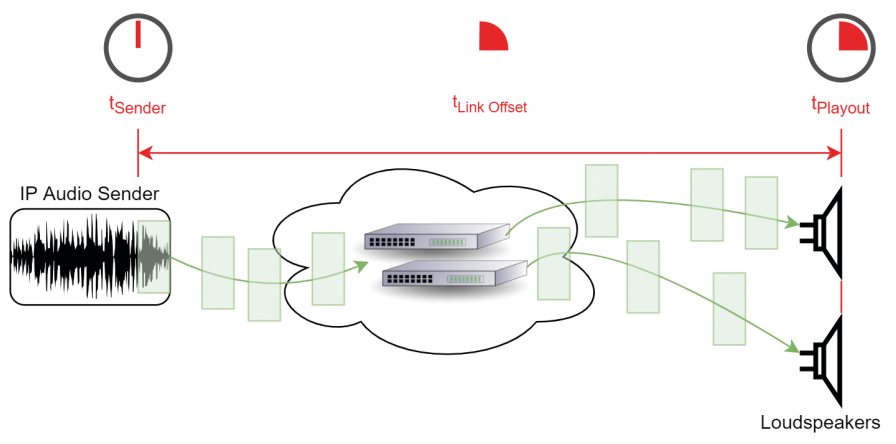
\includegraphics[width=\linewidth, keepaspectratio]{figures/phase_coherence_link_offset.png}
	\caption{Fáziskoherencia azonos kapcsolati eltolással \cite{AHNERT2023}}
	\label {fig:phase_coherence_link_offset}
\end{figure}
%----------------------------------------------------------------------------
\subsection{Szinkronizáció}
%----------------------------------------------------------------------------
Az IP-alapú küldők és fogadók szinkronizációja elengedhetetlen az alacsony késleltetéssel történő működéshez. 
A hagyományos audio technológiákban az eszközök szinkronizálása külön \textit{word clock} kapcsolatokkal 
vagy szinkronizált audioformátumokkal, például AES/EBU vagy MADI révén történt.

A fogadók közvetlenül ki tudják nyerni a frekvenciát és a fázist az ilyen formátumokból, mivel ezek 
biztosítanak egy \textit{impulzust}, amely jelzi, amikor egy audio minta létrejön vagy lejátszódik, például 
az analóg-digitális konverterek esetében. A PTP csomagok kis méretűek, és nem jelentős forgalmat 
generálnak, de elengedhetetlen, hogy a kapcsolók a lehető legmagasabb prioritással továbbítsák őket. 
Ez végső soron növeli a szinkronizáció pontosságát.

A QoS (Quality of Service) keretein belül a PTP csomagokat a hangadatoknál is magasabb prioritással kell kezelni. 
Az összes hálózati eszközt a Precision Time Protocol (PTP) segítségével szinkronizálják ugyanazon naptári időpontra. 
Az időreferencia egy olyan eszköztől származik, amelyet óraleadernek neveznek, míg az ehhez igazodó eszközöket óra követőknek hívják.

Minden eszköznek generálnia kell a kívánt hagyományos órát az abszolút időből, amelyet a PTP-n keresztül kapott. 
Ez a belső óra a \textit{médiaóra}. Ha a gyártó megfelelően implementálja, minden eszköz médiaórájának pontosan 
ugyanannak kell lennie frekvencia és fázis tekintetében. A magas pontosság technikailag elérhető, de kihívást 
jelent az audio gyártók számára. Ennek megfelelően a PTP szinkronizált eszközök közötti fázispontosság 
minőségtől függően változhat. Elfogadható eltérésnek tekinthető, ha az kisebb mint 1 µs (1 mikroszekundum).

Mivel az IT hálózatok nem rendelkeznek kellő determinisztikus jellemzőkkel a csomagok kézbesítésének időpontját 
illetően, a készülékek pontos szinkronizációja kifinomult megközelítést igényel. 
A PTP követők feladata két hatás kompenzálása, amelyek bármilyen hálózati környezetben előfordulhatnak:
%----------------------------------------------------------------------------
\subsubsection{Jitter kompenzáció}
%----------------------------------------------------------------------------
A PTP vezető által megadott jelenlegi időt a szinkronizációs üzenetekben az összes
követő egy ismert multicast címen (224.0.1.129) keresztül kapja. A hálózati
környezetből adódóan az információ nem mindig érkezik állandó késleltetéssel
a vevőkhöz. Ez a jelenség csomag jitter vagy csomag késleltetési változás (PDV)
néven ismert, amelyet minden PTP követőnek kompenzálnia kell. Az audio
hálózatok általában 1-8 üzenet/mp szinkronizálási arányt használnak, ahol a
nyolc üzenet csak kompatibilitás céljából ajánlott.

%----------------------------------------------------------------------------
\subsubsection{Késleltetés mérése}
%----------------------------------------------------------------------------
A követők egyik kulcsfontosságú feladata a csomagkésleltetés mérése a vezető
és a követő között, hogy korrigálják a szinkronizációs üzenetek időpontját.
Ehhez pontos időmérés szükséges, amely megmutatja, mennyi időbe telik egy
csomag átvitele a hálózaton. Ez a mérés tartalmazza a kábelek és kapcsolók
késleltetését is. A kábelhossz és a kapcsolók száma nem lényeges, csak a
végső késleltetés. A PTP időnek az összes követő között nanoszekundum pontossággal
ugyanannak kell lennie.

A PTP rendszerek számára alapvető, hogy a késleltetés mindkét irányban
állandó és szimmetrikus maradjon: a vezetőtől a követőig és vissza.
A késleltetést a követő két üzenet cseréjével méri: a késleltetési kérés
és a késleltetési válasz révén. Ezt általában a szinkronizálási aránnyal
azonos gyakorisággal végzik.

%----------------------------------------------------------------------------
A hálózaton több eszköz is képes lehet PTP vezetőként működni, ezért a
szabvány szabályokat határozott meg a vezető kiválasztására. Ezt a
szabályt a Best Master Clock Algorithm (BMCA) néven ismerjük, amely
a Legjobb Mesteróra Algoritmus.

Minden vezetőképes eszköz képes bejelentő üzeneteket küldeni
a prioritásairól és az oszcillátor pontosságáról. Ezenkívül figyelnie
kell a többi eszköz bejelentő üzeneteire is. Ha egy másik eszköz
jobb minőséget képvisel, az eszköz leállítja vezetőként való
bejelentkezését. Ellenkező esetben rendszeresen küldi saját
üzeneteit, mintegy \textit{szívverésként} jelezve aktív állapotát.

Ezeket az üzeneteket az announce intervallumnak nevezett időközönként
küldik el. A bejelentő üzenetek \textit{szívverésként} szolgálnak,
jelezve, hogy a jelenlegi mester még működőképes. Ha a kapcsolat
megszakad, az összes egység vár egy bizonyos időt (bejelentő időtúllépés),
amíg elküldik bejelentő üzeneteiket, majd újra végrehajtják a
kiválasztási folyamatot. A vezetőváltás idején a követőknek folytatniuk
kell saját oszcillátoruk működését, az audio lejátszás megszakítása
nélkül.

A bejelentő üzenetekben szereplő minőség két beállítható értéket tartalmaz:
prioritás 1 és prioritás 2. Mindkettő értéke 0 és 255 között változhat,
ahol a 0 a legjobb. Ha egy prioritás 1 érték kisebb egy eszközön,
mint a többi eszközön, az lesz a vezető. A prioritás 2 csak akkor
fontos, ha a prioritás 1 értékek megegyeznek több eszközön. Ez előfordulhat
két azonos típusú eszköz esetén, ahol a felhasználó ugyanazt az értéket
állította be a prioritás 1-hez. Ebben az esetben a prioritás 2 határozza
meg a fő vezetőt és a tartalékot.

Fontos megjegyezni, hogy néhány eszköz nem kínál lehetőséget a felhasználó
számára ezen értékek megadására. Ezek az eszközök a \textit{Preferált
Vezető} megjelöléssel rendelkeznek, amely rögzített értéket használ
bejelentő üzeneteikben, amit a gyártó határoz meg. Ennek ellenére
lehet, hogy egy alacsonyabb értéket megadva egy másik PTP vezető
felülbírálhatja ezt a típusú eszközt. Néhány eszköz támogatja a
\textit{Csak Követő} beállítást is, amely lehetővé teszi, hogy az
eszköz soha ne próbálja átvenni a vezetői szerepet a PTP hálózaton.

%----------------------------------------------------------------------------
\subsection{Mintavételi frekvencia és bitmélység}
%----------------------------------------------------------------------------
Az audio over IP rendszerek optimális működéséhez kulcsfontosságú a megfelelő mintavételi frekvencia
és bitmélység kiválasztása. E paraméterek jelentős hatással vannak az audio minőségére
és a hálózati teljesítményre. Fontos figyelembe venni az átviteli kapacitást, valamint
az eszközök maximális mintavételi frekvenciáját és bitmélységét. Ha a hálózat nem
képes biztosítani a szükséges sávszélességet, az instabilitást, hangkimaradást vagy
a hálózat teljes összeomlását okozhatja. Az audio rendszerekben gyakran alkalmazott
48 kHz-es mintavételi frekvencia széles hangsávot biztosít és kompatibilis a
számos professzionális hangtechnikai alkalmazással. Az utóbbi időben egyre szélesebb
körben elterjedt a 96 kHz-es mintavételi frekvencia, amely nagyobb részletességet
és jobb hangminőséget nyújt, viszont nagyobb sávszélességet igényel. A sávszélesség
kiszámításához az alábbi képlet használható:
%----------------------------------------------------------------------------
\begin{equation}
	\label{eq:sávszélesség}
	Sávszélesség\ igény = MintavételiFrekvencia \times BitMélység \times CsatornákSzáma
\end{equation}
%----------------------------------------------------------------------------
E formulával gyorsan meghatározhatjuk a szükséges sávszélességet. Például egy
64x64 csatornás rendszer, 96 kHz-es mintavételi frekvenciával és 24 bites
bitmélységgel a következő sávszélességet igényli:
%----------------------------------------------------------------------------
\begin{equation}
	\label{eq:sávszélesség}
	96000 \times 24 \times 64 \times 2 = 294912000\ bit/s = 294,912\ Mbit/s (\text{nyers adatfolyam})
\end{equation}
%----------------------------------------------------------------------------
A hálózat tervezésekor mindig szükséges némi tartalék, ezért a korábban említett
30 százalékos túlméretezést érdemes gyakorlatban is alkalmazni. Így a fenti
példa alapján a szükséges sávszélesség:
%----------------------------------------------------------------------------
\begin{equation}
	\label{eq:teljes-sávszélesség}
	294912000\ bit/s \times 1.3 = 383385600\ bit/s = 383,386\ Mbit/s (\text{teljes sávszélesség})
\end{equation}
%----------------------------------------------------------------------------
E számítások alapján egy 1 Gbit/s (1000 Mbit/s) sávszélességű hálózat elegendő
a rendszer zavartalan működéséhez, feltéve hogy az audio adatok kezelésére van
dedikálva. A bitmélység határozza meg a digitális hangminőséget, és az adatok
pontosságát. Az audio over IP területén jellemzően 16 vagy 24 bitmélységű rendszerek
terjedtek el, de a Dante rendszerek támogatják a 32 bites bitmélységet is. A 16
bites reprezentáció elegendő lehet olyan alkalmazásokhoz, ahol a dinamikatartomány
nem kritikus, míg a 24 bites felbontás pontosabb és részletesebb hangátvitelt
biztosít, ideális zenei stúdiókban és élőzenei környezetekben. A 32 bites
bitmélység a legmagasabb minőséget nyújtja, de nagyobb sávszélességet igényel,
így főként professzionális stúdiókban alkalmazzák. Általában azonban a 24
bites bitmélység bőven megfelel az elvárásoknak.

%----------------------------------------------------------------------------
\subsection{Késleltetés}
%----------------------------------------------------------------------------
Ha egy csomag például 1 ms hanganyagot tartalmaz, a kapcsolat késleltetése
mindig nagyobb lesz, mint 1 ms. A küldőnek először 1 ms hangot kell pufferelnie,
mielőtt az adatokat csomagba rendezi és elküldi. Ezt követően a csomag
hálózati utazása az összes kapcsolóval, mielőtt végül a fogadó eszköz pufferébe
érkezne, további késleltetést eredményez.

%----------------------------------------------------------------------------
\begin{enumerate}
    \item Csomag idő
    \item Utazási idő a hálózaton
    \item Fogadási puffer
\end{enumerate}
%----------------------------------------------------------------------------
A gyakorlatban a \textit{link offset} kifejezés azonos a késleltetés fogalmával.
A felhasználó feladata, hogy olyan link offsetet válasszon, amely elegendő
a fogadó puffer folyamatos telítettségének biztosítására, így elkerülhetők
a hangkimaradások.

%----------------------------------------------------------------------------
\subsection{IP-címek és maszkok}
%----------------------------------------------------------------------------
Hálózati környezetben minden eszköznek egyedi címre van szüksége, hogy a
csomagok célba érhessenek, és elkerülhetőek legyenek a csomagütközések.
Ez a cím lehet hardverrel kapcsolatos (MAC-cím) vagy konfigurálható (IP-cím).

%----------------------------------------------------------------------------
\section{IP-cím hozzárendelési módszerek}
%----------------------------------------------------------------------------
Az IP-címek hozzárendelése három módszer egyikével történhet:

%----------------------------------------------------------------------------
\begin{itemize}
    \item \textbf{Kézi beállítás:}
    Ez a módszer dokumentációt és felhasználói figyelmet igényel annak érdekében,
    hogy egy adott IP-címet csak egyszer használjanak egy hálózaton belül.
    Állandó telepítések esetén előnyös lehet, mivel könnyen nyomon követhető
    az IP-címek kiosztásának struktúrája.

    \item \textbf{DHCP szerver általi hozzárendelés:}
    Ez a rugalmas és strukturált módszer az IP-címek kiosztására a hálózaton belül.
    Egy eszköz „DHCP módban” próbálja megtalálni a DHCP szervert, és automatikusan
    beszerzi a szükséges IP-konfigurációkat. Az adminisztrátor beállíthatja a DHCP
    szervert úgy, hogy csak bizonyos IP-cím-tartományokat oszt ki, míg másokat
    kézi rendelésre tartalékol.

    \item \textbf{Önkiosztás:}
    Ezt a mechanizmust \textit{Zeroconfig} néven is ismerjük. Kisebb telepítések
    esetén használható, mivel az összes eszköz ugyanabban az alhálózatban van,
    és nem csatlakozhat más alhálózatokhoz.
\end{itemize}

%----------------------------------------------------------------------------
Egy eszköz IP-címének információja nehezen nyerhető ki, ha az nem jelenik meg
kijelzőn. Annak megállapítása, hogy két IP-cím azonos alhálózatba tartozik-e,
csak az alhálózati maszkok ellenőrzésével lehetséges. Ha a cél-IP-cím nem
ugyanabban az alhálózatban van, a csomagot a router IP-címére kell irányítani,
nem közvetlenül a fogadó eszközhöz. Két eszköz ugyanabban az alhálózatban
használhat hasonló IP-címeket, csupán az utolsó számjegyek eltérőek.
Az alhálózati maszk `0'-s számjegyei jelzik a hálózati és hosztcímek
szétválasztását. A hálózati címkét az alhálózati maszk `0'-nál nagyobb
értéke jelzi, míg a hosztcím a maradék rész, ahol az alhálózati maszk `0'-t
jelöl.

%----------------------------------------------------------------------------
\begin{figure}[H]
    \centering
    \begin{minipage}{0.45\textwidth}
        \centering
        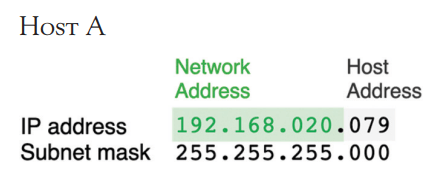
\includegraphics[width=67mm, keepaspectratio]{figures/host_a.png}
        \caption{Host A}
    \end{minipage}\hfill
    \begin{minipage}{0.45\textwidth}
        \centering
        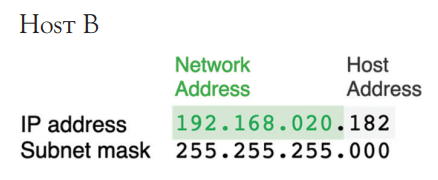
\includegraphics[width=67mm, keepaspectratio]{figures/host_b.png}
        \caption{Host B}
    \end{minipage}
\end{figure}

%----------------------------------------------------------------------------
Host A és Host B ugyanazon alhálózatba tartoznak, mivel azonos hálózati címkét
használnak (192.168.020). Az IP-cím hálózati része az a rész, ahol az
alhálózati maszk 255-ös értéket mutat. E két eszköz között router nem szükséges.

%----------------------------------------------------------------------------
\begin{figure}[H]
	\centering
	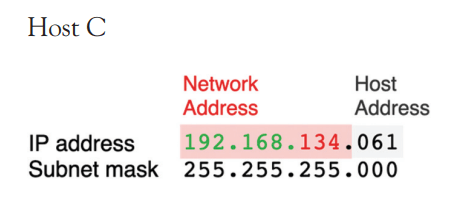
\includegraphics[width=67mm, keepaspectratio]{figures/host_c.png}
	\caption{Host C}
	\label {fig:host_c}
\end{figure}

%----------------------------------------------------------------------------
Host C eltérő alhálózatban található, mint Host A és B, mivel a hálózati cím
(192.168.134) eltér a többi eszköz címétől (192.168.020). Host C nem tud
csomagokat cserélni A és B eszközökkel router nélkül. Az eszköz kommunikációjához
más IP-címet kell kapnia, például 192.168.134\ldots címet, vagy más
alhálózati maszkot kell használni, például 255.255.0.0.

%----------------------------------------------------------------------------
Az alhálózati maszkok decimális jelölése dot-decimális formátumú. Az alternatív
módszer, a CIDR vagy perjeljelölés rövidebben reprezentálja az alhálózati maszkot,
a perjel után megadva az alhálózati maszk bitjeinek számát. Ez a jelölés az
alhálózati maszk bináris formáját tükrözi, ahol a `255' érték a `11111111'
binárisnak felel meg. Az előző példákban az alhálózati maszkok bináris formájukban
24 `1'-et tartalmaznak.

A fenti példában szereplő hosztok CIDR jelölése:

%----------------------------------------------------------------------------
\begin{itemize}
    \item \textbf{Host A:} 192.168.020.182/24
    \item \textbf{Host B:} 192.168.020.079/24
    \item \textbf{Host C:} 192.168.134.61/24
\end{itemize}
%----------------------------------------------------------------------------

A routerek használata és az alhálózatok összekapcsolása a hálózati rendszerek OSI modelljének harmadik rétegén alapul. 
Az OSI modell hét rétegre osztja a hálózati funkciókat, mindegyik réteg egy specifikus funkcionalitás halmazt ír elő a hálózati eszközöknél. 
Főként a csomagok célba juttatásáról van szó, ahol az eszközök a megfelelő címzett felé továbbítják az adatokat.

A modern informatikai eszközök ezt a jól definiált absztrakciós rétegmodellt követik, hogy biztosítsák az 
interoperabilitást a különböző gyártók között. Az OSI modell harmadik rétegén működő rendszerek képesek az 
IP-címek és alhálózati maszkok kezelésére, ami lehetővé teszi a csomagok alhálózatok közötti továbbítását. 
Az ilyen technológiák mindegyike ezen alapelvek szerint működik. Ezzel szemben léteznek olyan technológiák is, 
amelyek kizárólag a második réteg szintjén működnek.

Ezek a technológiák csak MAC-címek alapján képesek a csomagok továbbítására, alhálózati információk nélkül. 
Ennek következtében a második rétegű hálózatok nem oszthatók több alhálózatra, a csomagok nem továbbíthatók 
routerek által, így a skálázhatóságuk jelentősen korlátozott. Példaként említhetjük a már ismertetett 
TSN/Milan és CobraNet hálózati megoldásokat, amelyek a második réteg technológiákat alkalmazzák.

%----------------------------------------------------------------------------
\begin{figure}[H]
	\centering
	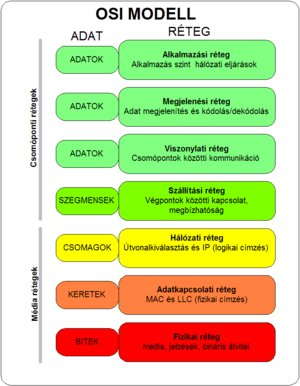
\includegraphics[width=150mm, keepaspectratio]{figures/osi_modell.jpg}
	\caption{Az OSI modell}
	\label {fig:osi_modell}
\end{figure}
%----------------------------------------------------------------------------

Az alhálózatok a hálózaton belüli logikai szegmensek, amelyek különböző indokok miatt jönnek létre, 
például adminisztratív és biztonsági okokból. A routerek lehetőséget biztosítanak az alhálózatok 
közötti összekapcsolásra, lehetővé téve ezzel a hosztok számára, hogy csomagokat cseréljenek anélkül, 
hogy elhagynák az alhálózati határokat. Fontos, hogy a hálózati útvonalak helyesen legyenek 
konfigurálva az alhálózatok közötti kommunikáció biztosítása érdekében. 
Ezzel szemben a klasszikus kapcsolók nem rendelkeznek azzal a képességgel, hogy az alhálózatokat összekapcsolják.

A virtuális LAN (VLAN) létrehozása egy alternatív módszert jelent a hálózat szegmentálására. 
Ez a megközelítés növeli a rendszer rugalmasságát és csökkenti a nem szükséges kommunikációt 
a nem kapcsolódó rendszerek között. A VLAN-ok nem csupán az alhálózatoknál biztonságosabb 
módszert nyújtanak a hosztok elválasztására, hanem további biztonsági előnyöket is biztosítanak.

%----------------------------------------------------------------------------
\subsection{Hálózati topológiák}
%----------------------------------------------------------------------------
A csomópontok összekapcsolási módjai eltérőek lehetnek, és a hálózat tervezésekor a
topológia kiválasztása az egyik legfontosabb döntés. A csillag topológia számos szempontból
előnyös megoldásnak bizonyul. Ebben a konfigurációban több hoszt csatlakozik egy központi
útválasztó eszközhöz, például kapcsolóhoz vagy routerhez. A mai modern hálózatok gyakran
két szintű csillag topológiát alkalmaznak, amelyet gerinc/levél architektúraként is
ismerünk. A központi kapcsoló vagy router (gerinc) általában nagyobb forgalmat
kezel, mint a perifériális kapcsoló (levél). Ha a gerinc és a levél közötti nagy
sávszélességű kapcsolat nem képes egyszerre kezelni az összes hoszt forgalmát, akkor
ez a tervezési forma blokkolóvá válhat. Ezzel szemben egy nem blokkoló hálózattervezés
esetén a nagy sávszélességű kapcsolatok képesek kezelni az összes csatlakoztatott hoszt
teljes forgalmát. A gyűrű topológia esetében a csomópontok közötti kapcsolatok száma
általában legalább kettő, és minden kapcsolat teljes sávszélességet biztosít. A csomópontok
feladata, hogy továbbítsák a csomagokat a gyűrűn belül, így minden csomópont olyan
szerepet tölt be, mint egy kapcsoló, amely a csomagokat két interfész között továbbítja.
A gyűrű topológia gyakran megfelelő választás lehet nagy távolságok áthidalására, különösen
akkor, ha a kapcsolatok költségesek. Gyakorlati példák közé tartoznak a különböző
helyszínek közötti hálózatok, valamint olyan eszközök csatlakoztatása, ahol nincs hely
további kapcsolók számára. A gyűrű topológiák beépített redundanciát nyújtanak, lehetővé
téve az eszközök elérését még akkor is, ha egy kapcsolat megszakad. A megfelelő hálózati
kialakításhoz elengedhetetlenek a nem blokkoló kapcsolók is. A nem blokkoló architektúra
azt jelenti, hogy a kapcsoló nem jelenti a szűk keresztmetszetet, így képes kezelni az
összes rá táplált forgalmat, ahol csupán a port sebessége képezheti a korlátot.


%----------------------------------------------------------------------------
\subsection{Unicast és Multicast} %Egyedi és Csoportos Küldés
%----------------------------------------------------------------------------

Amikor egy eszköz adatcsomagot küld egy másik eszköznek, unicast módszert alkalmaz. 
Ez a kommunikációs forma egyetlen küldőt és egyetlen fogadót jelent. Az unicast 
kapcsolatok gyakran a Transmission Control Protocol (TCP) révén történnek, ahol a
fogadó minden egyes csomag sikeres átvételéről visszaigazolást küld a küldőnek. Ha
a visszaigazolás nem érkezik meg, a küldő automatikusan újraküldi a csomagot. 
Alternatívaként az User Datagram Protocol (UDP) használata is lehetséges, ahol a
küldő feltételezi, hogy a csomagok sikeresen eljutnak a fogadóhoz. Ebben az esetben
nincs visszaigazolás, és ha a csomagok elvesznek, az adatok is elvesznek.
Ez az UDP megbízhatatlanságát jelenti? Valójában nem, csupán más alkalmazási 
esetre van optimalizálva. Bár meglepő lehet, de az UDP gyakran preferált az 
audio hálózatokban, ahol az alacsony késleltetés elengedhetetlen. Az újraküldés
időigényes lenne, ami növelné az általános késleltetést. Élő audio esetén a legjobb
megoldás az, ha folytatjuk a következő minták lejátszását anélkül, hogy próbálnánk
helyreállítani az elveszett adatokat. A kezelhető switchek és végpontok képesek
naplózni a csomagvesztéseket, lehetővé téve ezzel a hálózat állapotának monitorozását.

Az audio alkalmazások gyakran igénylik, hogy egy audio jel párhuzamosan több helyen
is megjelenjen, például egy mikrofonjel esetében, amelyet egyszerre továbbítanak
a front-of-house és a monitoring keverőpultokhoz, esetleg egy harmadik helyre
is, mint például egy felvevő eszköz. Ha a küldő unicast módban továbbítja a csomagokat,
az audio jel három különböző csomagban érkezik meg, azonos tartalommal, de eltérő
címekkel. Ez felesleges processzor terhelést okoz a küldő eszköz számára, és több
sávszélességet is igénybe vesz. Az optimalizálás érdekében a multicast módszer
alkalmazása javasolt, amely csökkenti a küldő eszközeinek processzor terhelését és
a hálózati forgalmat. A multicast címekre történő címzés lehetővé teszi, hogy a
küldő csupán egyszer helyezze el az audio adatokat egy csomagban, és azt egy multicast
címre küldje. A vevőknek csak annyit kell tudniuk, hogy mely multicast címre
akarnak figyelni. A multicast címek nem kapcsolódnak alhálózatokhoz vagy
IP-címekhez, így a multicast csomagok áthaladnak az alhálózatokon, ha nem
vannak VLAN-okkal elkülönítve. 

Ha a hálózat nem kizárólag audio jelek továbbítására van kialakítva, lehetnek olyan
eszközök is, amelyek nem kapcsolódnak az audiohoz. Ezért fontos, hogy a multicast
forgalom csak az érdeklődő hosztokhoz jusson el. Ezt az IGMP snooping (Internet
Group Management Protocol) segítségével érhetjük el. Az audio hálózati technológiák
általában támogatják az IGMP snooping-ot. Ha a kapcsolóban aktiválva van, akkor a
multicast csomagok csak azokon az interfészeken kerülnek továbbításra, ahol a
csatlakoztatott hosztok IGMP kéréseket küldenek. Ha nincs ilyen kérés, a multicast
leáll, elkerülve a felesleges forgalmat. Az IGMP snoopingot egy zsiliphez hasonlíthatjuk,
amely alapértelmezés szerint zárva van, és csak kérésre nyílik meg. Erősen ajánlott
az IGMP snooping aktiválása minden kapcsolóban egy multicast hálózatban. Fontos
azonban, hogy csak egy aktív IGMP Querier lehet a hálózatban, mivel az összes többi
kapcsoló tőle kapja az információkat. Ha nincs aktív IGMP Querier, a multicast
továbbítása broadcast formájában történhet, ami jelentős felesleges forgalmat
eredményezhet.

Összefoglalva, a unicast a legjobb késleltetési teljesítményt nyújtja, és a
kapcsolók számára a legkönnyebben kezelhető. Ezzel szemben a multicast jobb
sávszélesség-kezelést biztosít, különösen amikor a csatornaszám és a sávszélesség
növekszik.


%----------------------------------------------------------------------------
\subsection{Eszköz- és Adatfolyam-felfedezés}
%----------------------------------------------------------------------------

Az AES67 audió szabvány nem tartalmaz specifikációt arra vonatkozóan, hogyan
ismerhetik fel egymást a hálózati eszközök, illetve mely adatfolyamok állnak
rendelkezésre a hálózaton. A rendelkezésre álló technológiák közül mindegyik a
Bonjour vagy mDNS mechanizmust alkalmazza az eszközök értesítésére. Minden eszköz
fix multicast címet (224.0.0.251) használ, amelyre üzeneteket küld, hogy a
többi eszköz értesüljön a hálózaton belüli jelenlétéről. Ennek a mechanizmusnak
az egyik korlátja, hogy nem működik hatékonyan nagyobb telepítések esetén, ahol
több alhálózat vagy VLAN van jelen. Az ilyen helyzetek kezelésére a gyártók
saját megoldásokat dolgoztak ki (például Audinate Dante Domain Manager) vagy
követik az audio/video NMOS szabványt a felismerés és a kapcsolatkezelés terén.
Az audio adatfolyamok felfedezését a gyártótól függően két mechanizmus egyikével
valósítják meg. Az eszközök felfedezéséhez hasonlóan mindkét esetben előre
meghatározott multicast címet alkalmaznak az adatfolyam-információk
terjesztésére, hogy a címzettek rátaláljanak az elérhető adatfolyamokra és azok
paramétereire:

%----------------------------------------------------------------------------
\begin{itemize}
	\item Session Announcement Protocol (SAP) - minden Dante termék használja (Multicast cím: 239.255.255.255)
\end{itemize}

\begin{itemize}
	\item Bonjour / mDNS - minden más technológia alkalmazza (Multicast cím: 224.0.0.251) 
\end{itemize}
%----------------------------------------------------------------------------
Szerencsére a legtöbb modern termék lehetővé teszi mindkét protokoll egyidejű
aktiválását, így egy adott audio adatfolyam párhuzamosan bejelenthető mindkét
mechanizmuson keresztül.

%----------------------------------------------------------------------------
\subsection{Redundancia}
%----------------------------------------------------------------------------

Az audiohálózatok korai időszakaiban néhány felhasználó kétségekkel
tekintett az IT hardverek megbízhatóságára. Annak ellenére, hogy az IT-berendezések
széleskörű alkalmazása során gyakran bizonyították megbízhatóságukat, és
sok esetben még a hagyományos audioberendezéseknél is jobb teljesítményt nyújtanak,
továbbra is fontos a redundancia biztosítása. Az IT-hálózati komponensek általában
több diagnosztikai eszközt kínálnak, amelyek lehetővé teszik a hibák gyors
felismerését és kezelését.


%----------------------------------------------------------------------------
\subsubsection{Spanning Tree Protocol (STP)}
%----------------------------------------------------------------------------

Amikor a kapcsolókat úgy konfigurálják, hogy hurkot alkossanak, fennáll a
veszélye annak, hogy a csomagok végtelen ciklusban keringenek a hurokban. 
Ezt a problémát a hálózati hardver automatikusan észleli az STP (Spanning Tree Protocol)
segítségével. Az STP a hurok detektálása esetén automatikusan letilt egy kapcsolatot. 
Az STP nemcsak a hurok jelenség kezelésére használható, hanem a véletlenszerű 
kapcsolatvesztések, például kábelvágások esetén is nyújt védelmet.

A mechanizmus szándékosan hoz létre hurkokat, majd, ha egy kábel véletlenül
kiesik, a rendszer gyorsan észleli ezt, és aktiválja a passzív kapcsolatot. 
Ez a folyamat néhány másodperces audio megszakítást eredményezhet, azonban
ez még mindig jelentősen gyorsabb, mint a manuális hibaelhárítás és új kábel
telepítése. Az STP alapértelmezetten engedélyezett a legtöbb rendszerben.
Enélkül broadcast "viharok" keletkeznének, amelyek jelentős sávszélesség-veszteséget
és hálózati túlterhelést okoznának.

%----------------------------------------------------------------------------
\subsubsection{Link Aggregáció}
%----------------------------------------------------------------------------

Ha egy kapcsolat különösen kritikus egy telepítés során, akkor két vagy több kábelt
párhuzamosan lehet csatlakoztatni a megbízhatóság növelése érdekében. 
A link aggregáció elsődleges célja a sávszélesség növelése két kapcsoló között.
Ezen kívül költséghatékony megoldást nyújt a kapcsolat véletlen leválasztása vagy
kábelvágás esetén. Például egy színpad, amely egy keverőhöz csatlakozik, gyakran
alkalmazza ezt a megközelítést. A kapcsolóknak mindkét végén azonos konfigurációra
van szükség: két vagy több interfészt Link Aggregációs Csoportként kell kijelölni,
amelyek egyetlen interfészként jelennek meg a kapcsolóban. Gyakorlatban a link
aggregáció segíthet csökkenteni a kábelproblémákat. Az egyszerűsége miatt a felhasználónak
csak egy további kábelt kell biztosítania és konfigurálnia kell a kapcsolókat mindkét
oldalon. Azonban a kábel leválasztása esetén az audioátvitel néhány másodpercig megszakadhat,
mielőtt a kapcsoló aktiválja az alternatív kapcsolatot.

%----------------------------------------------------------------------------
\subsubsection{Adatfolyam redundancia}
%----------------------------------------------------------------------------

A legbiztonságosabb, de legdrágább módja a redundancia biztosításának egy hálózatban
az, ha két teljesen független audiohálózatot építenek ki, amely két különálló utat
biztosít a küldő és a fogadó között. Ebben a konfigurációban minden csomópontnak
két hálózati interfészt kell rendelkezésre bocsátania. A küldő két azonos audio tartalommal
rendelkező csomagot generál, mindkettőre azonos PTP-időbélyeget alkalmaz, majd elküldi
mindkét hálózaton keresztül. A fogadó végén mindkét csomagot fogadják és feldolgozzák.
Még ha az egyik csomag elveszik is, a megmaradt csomag tartalmazza az összes szükséges
információt, és biztosítja az audio zavartalan folytatását. Ez a mechanizmus az egyetlen
módja a véletlenszerű csomagvesztés kompenzálásának anélkül, hogy a küldőtől újraküldés
által késleltetést okozna a rendszerben.

%----------------------------------------------------------------------------
\section{AES67}
%----------------------------------------------------------------------------

Az AES67 szabvány szerint minden eszköznek teljesítenie kell a következő alapvető követelményeket:

%----------------------------------------------------------------------------
\begin{itemize}
	\item Unicast és multicast kommunikáció támogatása
	\item UDP/RTP protokollok alkalmazása
	\item DSCP címkék beállítása előírt értékekre, QoS támogatás
	\item Nincs előírt automatikus eszköz- és adatfolyam-felfedezés
	\item PTPv2 szabvány használata az időszinkronizációhoz
	\item PTP profil: Standard (a gyakorlatban a Dante magasabb szinkronizációs rátát igényel)
	\item Küldőknek SDP fájlt kell generálniuk
	\item A fogadóknak képesnek kell lenniük SDP fájlok értelmezésére
	\item A fogadóknak legalább 3 ms hangpufferrel kell rendelkezniük
	\item Adatfolyam formátumok
	\item 1-8 csatorna (a küldő választhat fix számot, a fogadóknak viszont rugalmasnak kell lenniük)
	\item 24 bites és 16 bites felbontás (a küldő választ, de a fogadóknak mindkettőt kezelniük kell)
	\item 48 kHz mintavételi frekvencia, 1 ms csomagidő (48 mintával)
	\item Multicast címek: 239.0.0.0 és 239.255.255.255 között
\end{itemize}

A szabvány további paramétereket és értékeket is tartalmaz, azonban ezek nem
tartoznak a fent említett minimális követelmények közé.

%----------------------------------------------------------------------------
\section{Audinate Dante}
%----------------------------------------------------------------------------
\subsection{A Dante hálózatok áttekintése}
%----------------------------------------------------------------------------

A 2020-2021-es Covid-19 járvány során lehetőségem nyílt részt venni egy átfogó Dante
kurzuson, amelyet a Dante technológia fejlesztője, az Audinate szervezett. A kurzus
részletes betekintést nyújtott a Dante hálózatok működésébe. E fejezetben a belsős
oktatóanyagokat fogom felhasználni, amelyeket a kurzus alatt kaptam. Ezek a dokumentumok
csak a kurzus résztvevői számára elérhetők, így nem publikálhatók.

A Dante hanghálózatok digitális hangátviteli technológiát képviselnek, amely lehetővé teszi
a hang elosztását és irányítását szabványos Ethernet hálózatokon keresztül. Az ausztrál
Audinate vállalat által kifejlesztett Dante technológia az IP hálózatokat használja a
magas minőségű, alacsony késleltetésű hangátvitelhez az eszközök között. Ez a rendszer
nagyobb rugalmasságot és skálázhatóságot biztosít a hagyományos analóg hangrendszerekhez
képest, valamint lehetővé teszi a hangrendszerek integrálását meglévő IT infrastruktúrába.
A Dante hanghálózatok széles körben alkalmazottak, beleértve a koncerthangosítást, rádiózást,
stúdiófelvételeket, vállalati környezeteket és konferenciaközpontokat. A technológia
több hangformátumot és mintavételi rátát támogat, és akár több száz hangcsatorna egyidejű
átvitelét is lehetővé teszi egyetlen hálózaton keresztül. Emellett a Dante rendszerek távolról
vezérelhetők és monitorozhatók, amely megkönnyíti a komplex hangrendszerek beállítását és
kezelését.


%----------------------------------------------------------------------------
\subsection{Dante hálózatok technikai részletei}
%----------------------------------------------------------------------------
A Dante hanghálózatok két fő komponensből állnak: Dante eszközökből
és Dante hálózatokból. A Dante eszközök olyan hangeszközök, amelyeket
kifejezetten a Dante protokollhoz terveztek, mint például hangkártyák, erősítők
és hangládák. Ezeket az eszközöket szabványos Ethernet kábelekkel és
kapcsolókkal lehet csatlakoztatni a Dante hálózathoz.
A hálózatot az Audinate Dante Controller szoftverrel lehet
konfigurálni, amely lehetővé teszi a hang elosztását és útválasztását az
eszközök között. A szoftverrel tudjuk az eszközöket távoli vezérléssel elérni és
monitorozni a hálózaton. Ezek a hanghálózatok támogatnak számos
hangformátumot és mintavételi rátát, és képesek egyszerre több száz hangcsatorna
átvitelére egyetlen hálózaton keresztül. A technológia továbbá támogat olyan
fejlett funkciókat, mint a Dante Domain Manager (DDM) a biztonságos
hangátvitelhez, valamint a Dante Virtual Soundcard (DVS) a számítógépes alapú
hanglejátszáshoz és felvételhez. 

Tegyük fel, hogy több eszköz is küld hangot egy adott végpontra a hálózaton.
Alapesetben, ahogy a csomagok felgyülemlenek, az elsőként érkezőket, elsőként szolgálják ki elvet alkalmazzák.
A Dante hanghálózatok Quality of Service (QoS)
támogatást is nyújtanak, a prioritások kezelésére.
Ezzel biztosítható a hangátvitel elsőbbse más hálózati forgalommal szemben. Ez segít minimalizálni a hálózati
torlódás lehetőségét és biztosítani, hogy a hangátvitel minimális késleltetéssel
és magas minőségben történjen. 
Körülbelül 70 százalékos hálózati szaturációnál már ajánlott a QoS használata.
Valamint 100 Mbps-es hálózatoknál segít a jitter csökkenésében.

%----------------------------------------------------------------------------
\subsubsection{Több mintavételi ráta és bitmélység}
%----------------------------------------------------------------------------

A rendszer képes egyidejűleg több bitmélységet kezelni. Ennek informatikai háttere a
a következő képpen néz ki. Ha egy 32 bites hangforrásunk van, de a másik eszköz
csak 24 bites hangot tud fogadni, akkor a Dante a 32 bites hangot 24 bitesre tudja 
alakítani.

%----------------------------------------------------------------------------
\begin{align*}
	\begin{array}{|c|c|}
	\hline
	\text{Hangminták} & \text{Bitmélység} \\
	\hline
	\text{11110000 11110000 11110000 11110000} & \text{32 bites} \\
	\hline
	\text{11110000 11110000 11110000} & \text{24 bites} \\
	\hline
	\end{array}
\end{align*}
%----------------------------------------------------------------------------
	
Amint a példában látszik, 32 bites hangból úgy kaptunk 24 bites hangot, 
hogy egyszerűen csak elhagytuk az utolsó 8 bitet. Ez a folyamat visszafelé is működik,
ha 24 bites hangot kell 32 bites hanggá alakítani, akkor az utolsó 8 bitet 0-val kell feltölteni.

%----------------------------------------------------------------------------	
\begin{align*}
	\begin{array}{|c|c|}
	\hline
	\text{Hangminták} & \text{Bitmélység} \\
	\hline
	\text{11110000 11110000 11110000} & \text{24 bites} \\
	\hline
	\text{11110000 11110000 11110000 00000000} & \text{32 bites} \\
	\hline
	\end{array}
\end{align*}
%----------------------------------------------------------------------------

Mintavételezési frekvencia eltérést csak abban az esetben tudja kezelni, ha a
bitmélység is eltérő. Amennyiben a bitmélység azonos, de a mintavételezési
frekvencia eltérő, akkor a rendszer nem képes a hangot továbbítani.
Ez a mechanizmus egy egyszerű mechanikai példával jól megérhető és leírható.
Tegyük fel van két fogaskerekünk. Amennyiben a mintavételezési frekvencia azonos, és a 
bitmélység eltérő, akkor a fogaskerekek egymásba illeszthetőek és csak a fogaskerekek
mélysége fog eltérni. Amennyiben a mintavételezési frekvencia eltérő, akkor a fogaskerekek
nem illeszthetőek egymásba, és nem tudjuk továbbítani a hangot. Ebben az esetben már egy
konverterre lesz szükségünk, amely képes a két fogaskereket összeilleszteni számunkra.
Egy fontos kitétel van ahhoz, hogy a több mintavételi ráta egyszerre megfelelően működjön,
az pedig az egységes órajel az összes mintavételi frekvenciához.

%----------------------------------------------------------------------------
\subsubsection{Hálózati topológiák}
%----------------------------------------------------------------------------
A Dante rendszerek alapvetően kétféle módban tudnak üzemelni. Az első a
switched (kapcsolt) mód, amelyben az eszközökön található két Ethernet port
egy hálózatot alkot. Ebben a módban tudunk Daisy Chain (füzéres) topológiát kialakítani,
amelyben az egyik eszköz a másikhoz csatlakozik, és így tovább. Továbbá csillagtopológiát
is kialakíthatunk, amelyben minden eszköz egy központi kapcsolóhoz csatlakozik.
%----------------------------------------------------------------------------
\begin{figure}[H]
	\begin{minipage}{0.5\textwidth}
		\centering
		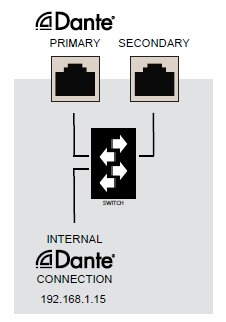
\includegraphics[width=100px, keepaspectratio]{figures/dante-switched-mode.jpg}
		\caption{Kapcsolt mód}
		\label{fig:dante_switched}
	\end{minipage}%
	\begin{minipage}{0.5\textwidth}
		\centering
		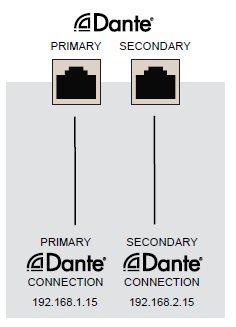
\includegraphics[width=100px, keepaspectratio]{figures/dante-redundant-mode.jpg}
		\caption{Redundáns mód}
		\label{fig:dante_redundant}
	\end{minipage}
\end{figure}

%----------------------------------------------------------------------------
A másik mód a redundant (redundáns) mód, amelyben az eszközökön található két
Ethernet port két különálló hálózatot alkot. Ebben a módban a hálózat redundáns
kialakítású, és a hálózat egyik része automatikusan átveszi a másik rész szerepét,
ha az meghibásodik.
Néhány Dante eszköznek létezik egy harmadik Ethernet portja, amelyet konfigurálási
és vezérlési célokra használnak.
%----------------------------------------------------------------------------
\subsubsection{Késleltetés}
%----------------------------------------------------------------------------
A késleltetés az az idő, amely szükséges egy folyamat végrehajtásához. Például
az idő amíg a bemeneti oldalon egy hangjel feldolgozásra kerül, és a kimeneti
oldalon megjelenik. 
Két fő mértékegységet használunk a késleltetés mérésére:
%----------------------------------------------------------------------------
\begin{equation}
	\label{eq:milliseconds}
	1 \text{ másodperc} = 1000 \text{ milli másodperc}, \quad \text{azaz} \quad 1 \text{ ms} = 0.001 \text{ s}
\end{equation}
%----------------------------------------------------------------------------
%----------------------------------------------------------------------------
\begin{equation}
	\label{eq:microseconds}
	1 \text{ másodperc} = 1000000 \text{ mikro másodperc}, \quad \text{azaz} \quad 1 \mu\text{s} = 0.000001 \text{ s}
\end{equation}
%----------------------------------------------------------------------------
A Dante eszközök lehetővé teszik a késleltetés teljesítményének meghatározását. 
A 0.1 milliszekundumos késleltetés az a késleltetés, amely már kapcsoló lépés biztos.
Ha két eszköz különböző késleltetésű, akkor a nagyobb érték lesz az irányadó.
Egy megfelelően konfigurált modern Dante hálózatban a késleltetés 1 ms körüli értéket vesz fel.
Ez azt is jelenti, hogy például egy dobos előbb hallja a hangszerét a fülmonitoron, mint a saját dobját.

%----------------------------------------------------------------------------
\subsubsection{Órajel}
%----------------------------------------------------------------------------

Minden eszköz egy nagyon-nagyon pontos Dátum/Idő órát követ.
Szinkronizálnak az időhöz és állítják a sebességet, hogy egységes legyen.
Mi a helyzet a terjedési késéssel? Miért vannak szinkronban a Dante eszközök?
A PTP (Precision Time Protocol) késleltetési kéréseket (Delay Requests)
ad ki, amelyek kiszámítják a hálózat késleltetését. 
Az eszközök az információváltás késését is kompenzálják.
A Dante automatikusan választ óra vezetőt.
Mindig csak egy óra vezető lesz, függetlenül a mintavételi rátától.
Beállíthatunk külső óra vezetőt is amennyiben szükséges.
Nem szinkronizál újra, hanem beállítja a sebességet és kompenzálja a hálózati késést.
A Dante által végzett tesztelések és tapasztalatok alapján
bebizonyosodott, hogy az időzítés szinkronban marad akkor is,
ha az óra perceken keresztül teljesen eltűnik.

%----------------------------------------------------------------------------
\begin{figure}[H]
	\centering
	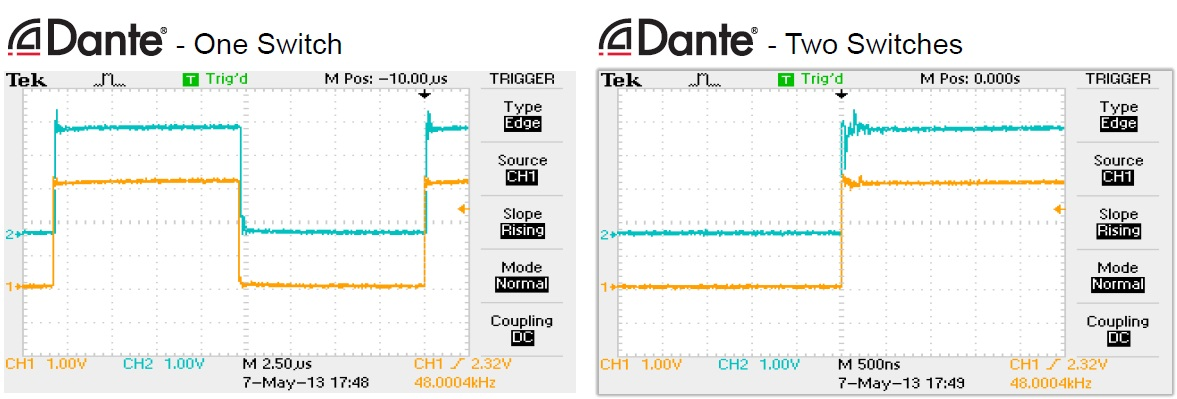
\includegraphics[width=400px, keepaspectratio] {figures/dante-clocking.jpg}
	\caption{Dante órajel}
	\label{fig:dante-clock}
\end{figure}
%----------------------------------------------------------------------------

%----------------------------------------------------------------------------
\subsection{Összehasonlítás a hagyományos hangrendszerekkel}
%----------------------------------------------------------------------------
A hagyományos hangrendszerek általában analóg kábelekre és csatlakozókra
támaszkodnak a hangjelek eszközök közötti átviteléhez. Ezek a rendszerek
korlátozottak lehetnek rugalmasságban, skálázhatóságban és az egyidejűleg
átvihető hangcsatornák számában. Emellett hajlamosak bonyolultabbá válni a
beállítás és kezelés szempontjából, mivel minden hangcsatornához külön kábel és
csatlakozás szükséges. A Dante hanghálózatok jóval több hangcsatornát is támogatnak,
mint a hagyományos analóg rendszerek, lehetővé téve a nagy, összetett hangrendszerek könnyű
beállítását és kezelését. A Dante hanghálózatok további előnye, hogy képesek
hangot továbbítani hosszú távolságokon anélkül, hogy a minőség romlana. A
hagyományos analóg rendszerek zajra és jelveszteségre hajlamosak hosszú kábelek
esetén, míg a digitális hangjelek, amelyeket az Ethernet hálózatokon
továbbítanak, minimális minőségveszteséggel juthatnak el nagy távolságokra.
%----------------------------------------------------------------------------
\begin{table}[htbp]
    \centering
    \caption{Digital Snake és DigitalAVNetwork Jelút opciók}
    \begin{tabular}{@{}lll@{}}
        \toprule
        \textbf{Kérdés} & \textbf{Pont-pont között} & \textbf{Hálózati megoldás} \\ \midrule
        Hová megy a jel? & Lineáris kábelút & Bárhol a hálózaton \\
        Hogyan változtassuk meg a jelútvonalat? & Mozgassuk a kábelt & Egy egérkattintással \\
        Szétválaszthatjuk-e a jeleket? & Nem & Igen - a hálózaton \\
        Megosztható-e a kábel más jelekkel? & Nem & Igen - közös infrastruktúra \\
        \bottomrule
    \end{tabular}
    \label{tab:digital-snake-vs-digitalavnetwork-hu}
\end{table}
%----------------------------------------------------------------------------
\begin{figure}[H]
	\centering
	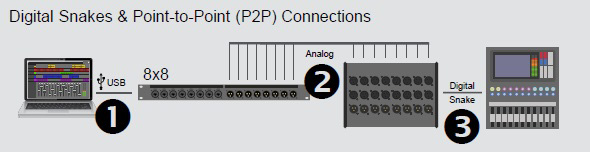
\includegraphics[width=\linewidth, keepaspectratio]{figures/dsnake-p2p.jpg}
	\caption{Digital Snake és Pont-pont közötti (P2P) kapcsolatok}
	\label {fig:dsnake-p2p}
\end{figure}
%----------------------------------------------------------------------------
\begin{figure}[H]
	\centering
	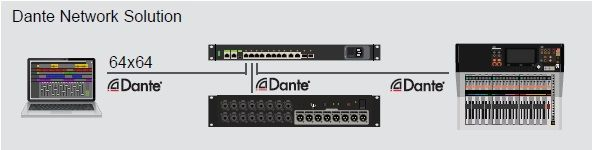
\includegraphics[width=\linewidth, keepaspectratio]{figures/dante-solution.jpg}
	\caption{Dante hálózati megoldás}
	\label {fig:dante-solution}
\end{figure}
%----------------------------------------------------------------------------

A rugalmasság és a skálázhatóság tovbbi kulcsfontosságú előnye a Dante
hanghálózatoknak a hagyományos analóg hangrendszerekkel szemben.
Képesek alkalmazkodni különböző hangkonfigurációkhoz és követelményekhez. 
Könnyű eszközöket hozzáadni vagy eltávolítani, megváltoztatni a hangjelek útvonalát, és a rendszert újra
konfigurálni szükség esetén. Ez lehetővé teszi testreszabott audio-megoldások
létrehozását, amelyeket az adott alkalmazás vagy környezet speciális igényeihez
lehet igazítani. 

%----------------------------------------------------------------------------
\subsection{Firmware frissítés}
%----------------------------------------------------------------------------

A Dante eszközök rendelkeznek Dante Firmware és Eszköz Firmware-el.
Lehet, hogy mindkettőt frissíteni kell. Kérjük, forduljon a gyártóhoz a párosított verziókért.
Néhány eszköz sorozat más módszerekkel frissíthető.
A Dante Updater hasznos lehet a frissítések nyomon követéséhez és telepítéséhez.
A rendszer ellenőrzi az online adatbázisunkat, hogy tájékoztassa Önt az elérhető frissítésekről.
A Dante firmware könnyen frissíthető.
A Dante Firmware Update Manager továbbra is aktuális.
Importálja a firmware fájlokat, ha firmware-t kap egy gyártótól.
Ha a frissítés nem sikerül, rendelkezünk vészhelyzeti helyreállítási módszerrel.
A Dante eszközök erős támogatást nyújtanak a vegyes firmware verziókhoz.
Mérnökeink automatizált regressziós tesztelést végeztek a korábbi firmware kiadásokkal szemben.

%----------------------------------------------------------------------------
\subsection{Chipek}
%----------------------------------------------------------------------------

A Dante hálózatok változatos chipekkel építhetők fel. 
Az Audinate számos különböző chipet kínál a Dante hálózatok létrehozásához, 
melyek eltérő hangcsatorna-számot és egyéb funkciókat támogatnak. 
A Dante chipek különféle méretekben és árkategóriákban elérhetők, 
lehetővé téve a gyártók számára, hogy különféle méretű és árú Dante 
eszközöket fejlesszenek ki, így képesek kielégíteni a különböző piaci igényeket. 
A Dante chipek segítik a gyártókat abban, hogy gyorsan és hatékonyan hozzanak 
létre Dante-kompatibilis eszközöket, és könnyedén integrálják azokat a saját termékeikbe.

%----------------------------------------------------------------------------
\begin{center}
	\begin{tabular}{|c|p{10cm}|}
		\hline
		\textbf{Chip} & \textbf{Leírás} \\
		\hline
		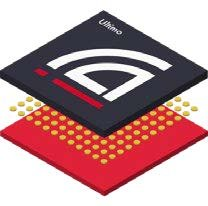
\includegraphics[width=40px,height=40px,keepaspectratio]{figures/ultimo-x.jpg} & \textbf{Dante Ultimo-X} - 0x4, 2x2, 4x0 \\
		\hline
		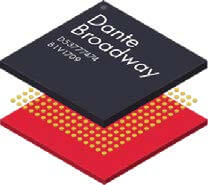
\includegraphics[width=40px,height=40px,keepaspectratio]{figures/broadway.jpg} & \textbf{Dante Broadway} - 16x16 \\
		\hline
		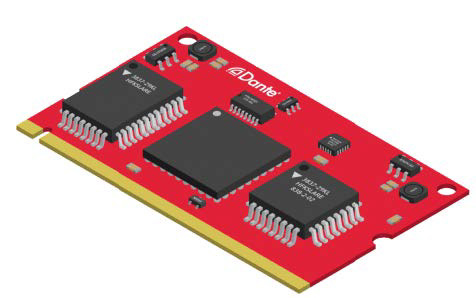
\includegraphics[width=40px,height=40px,keepaspectratio]{figures/brooklyn-ii.jpg} & \textbf{Dante Brooklyn II} - 64x64 \\
		\hline
		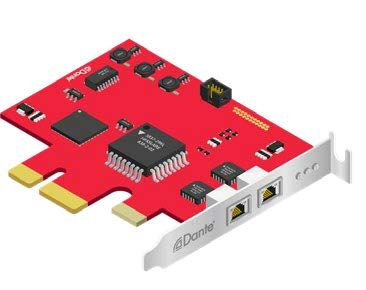
\includegraphics[width=40px,height=40px,keepaspectratio]{figures/pcie-r.jpg} & \textbf{Dante PCIe-R} - 128x128 \\
		\hline
		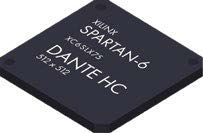
\includegraphics[width=40px,height=40px,keepaspectratio]{figures/dante-hc.jpg} & \textbf{Dante HC (High Capacity)} - 512x512 \\
		\hline
		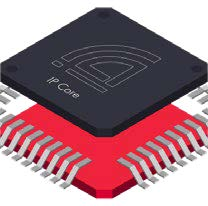
\includegraphics[width=40px,height=40px,keepaspectratio]{figures/shared-processor.jpg} & \textbf{Dante Shared Processor} - IP Core 512x512 FPGA and Dante Embedded Platform 64x64 X86/ARM \\
		\hline
		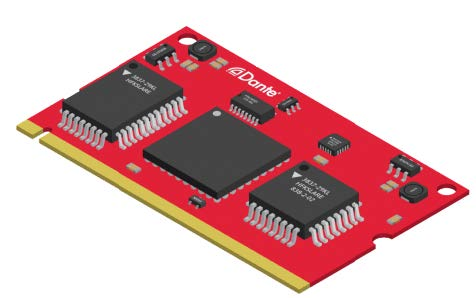
\includegraphics[width=40px,height=40px,keepaspectratio]{figures/dante-av.jpg} & \textbf{Dante AV} - V:1, A:8 \\
		\hline
	\end{tabular}
\end{center}
%----------------------------------------------------------------------------
	





